\subfloat[\label{fig:SousAlt_Metrique_1}]{
  \begin{tikzpicture}[remember picture,inner sep=0pt,outer sep=0pt]
    \tikzset{et/.style={above,font=\footnotesize\vphantom{Ag}}}
    \node[anchor=south west] (img)
    {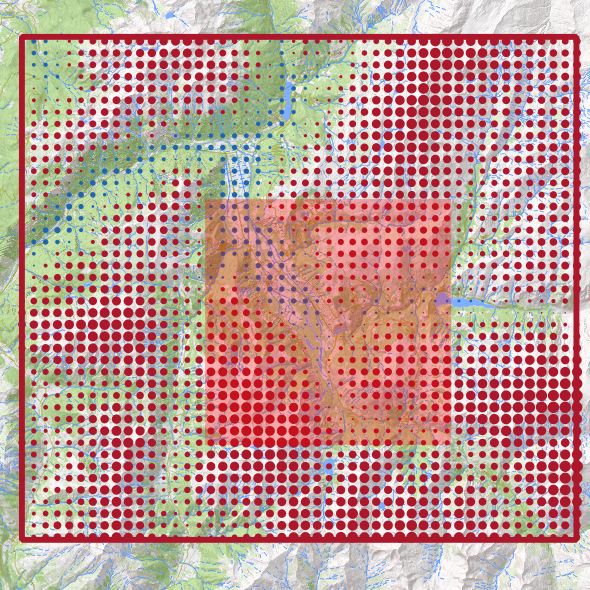
\includegraphics{../figures/ZLC_Sous_Chemin_1/ZLC.png}};
    \begin{scope}
      \node (P2) at ([yshift=-.5cm]img.south east) {};
      \node (P1) at ([yshift=-.5cm]img.south west) {};
      \draw[-] (P2 |- -1cm,-1cm) --++ (-1,0) node[et,pos=.5] {\SI{6}{\kilo\meter}};
    \end{scope}
    \begin{scope}[x=(img.south east),y=(img.north west)]
      \node[draw,RdBu-9-1,thick,minimum height=2cm,minimum width=2.00cm] (B1) at (0.53,0.46) {};
    \end{scope}
  \end{tikzpicture}
}\hspace{1cm}
%
\subfloat[\label{fig:SousAlt_ZLC_1}]{%
  \begin{tikzpicture}[remember picture,inner sep=0pt,outer sep=0pt]
    \tikzset{et/.style={above,font=\footnotesize\vphantom{Ag}}}
    \node (img1)
    {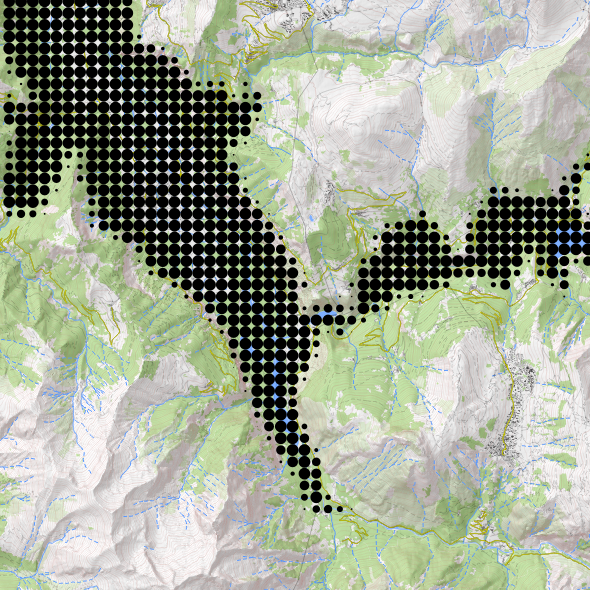
\includegraphics{../figures/ZLC_Sous_Chemin_1/ZLC_2.png}};
    \draw[-] ([yshift=-1cm]img1.south east) --++ (-1,0) node[et,pos=.5] {\SI{2,5}{\kilo\meter}};
    \draw[RdBu-9-1,thick,draw] (img1.south west) rectangle (img1.north east);
  \end{tikzpicture}
}
%
\begin{tikzpicture}[overlay, remember picture,RdBu-9-1,thick,draw,inner sep=0pt,outer sep=0pt]
  \draw (B1) -- (img1);
\end{tikzpicture}
